%   MSc Business Analytics Dissertation
%
%   Title:     Aaa Bbbbbbb Cccccccccc
%   Author(s): Xxxxxx Xxxxxxxxx and Yyy Yyyyyyyyy
%
%   Chapter 5: Results
%
%   Change Control:
%   When     Who   Ver  What
%   -------  ----  ---  --------------------------------------------------------------
%   11Feb11  AB    0.1  Begun 
%

\chapter{Results}\label{C.Results}

\section{Overview}
Model prediction accuracy of original test data set was 99.65\%, which is practically impossible. As discussed in chapter \ref{C.intro} actual data received from KPMG was made up using pre-defined formulas and rules to make it look real. Data didn't cover all possible scenario for a loan portfolio and achieving an accuracy of 99\% in credit scoring model is difficult as one needs to train model recursively with large data size covering all permutations and combinations of situations for loan default.

\section{Data Normalization}\label{S.intro5}

Original data set consist of 237389 observations and 35 variables, according to data 5\% of loan applications have defaulted, and the customer has credit rating 1 will not default ever. Therefore, to consider all possible scenarios data has been normalised, and a data subset has been generated from original data set to carry experiments.\\

In Table \ref{table:dataorg}, it is evident that data is very well structured and it does not give much information about the applicants who can default in future even if they had an excellent credit history. So loan portfolios of credit rating 1,2 and 3 don't contribute much to the objective of the project. Also, it can be seen that as per the distribution of original data, the only applicant with credit rating 5 will default. And this information does not comply to the real world scenarios. In discussion with KPMG, loan portfolios were again analysed to establish data that resembles the real world. Based on the variables such as loan balances, unemployment rates, annual income, address and mortgage years, changes had been made to the data that can be seen in Table \ref{table:datanormalized}. After data normalization, all cases are considered including some of the extreme cases; normalised data gives a better representation of loan portfolios accordance to real world with 0.22\% probability of default with credit rating 1, almost 11\% defaulters with credit rating 4 and 10\% chances of default and 1\% chance of not default in credit rating 5.   

% Please add the following required packages to your document preamble:
% \usepackage{booktabs}
\begin{table}[!htb]
\centering
\caption{Distribution of Defaulted Loans vs Credit for Original Data}
\label{table:dataorg}
\begin{tabular}{@{}ccc@{}}
\toprule
\multicolumn{1}{l}{\textbf{}} & \multicolumn{2}{l}{\textbf{Defaulted Loan?}} \\ \midrule
\textbf{Credit Rating}        & \textbf{Yes}          & \textbf{No}          \\ \midrule
\textbf{1}                    & 44.93\%               & 0\%                  \\ 
\textbf{2}                    & 21.24\%               & 0.01\%               \\ 
\textbf{3}                    & 17.40\%               & 0.01\%               \\ 
\textbf{4}                    & 10.96\%               &                      \\ 
\textbf{5}                    & 0.89\%                & 4.57\%               \\ \bottomrule
\end{tabular}
\end{table}

\begin{table}[]
\centering
\caption{Distribution of Defaulted Loans vs Credit for Normalized Data}
\label{table:datanormalized}
\begin{tabular}{@{}ccc@{}}
\toprule
\multicolumn{1}{l}{\textbf{}} & \multicolumn{2}{l}{\textbf{Defaulted Loan?}} \\ \midrule
\textbf{Credit Rating}        & \textbf{Yes}          & \textbf{No}          \\ \midrule
\textbf{1}                    & 25.71\%               & 0.22\%               \\ 
\textbf{2}                    & 20.95\%               & 0.79\%               \\ 
\textbf{3}                    & 17.27\%               & 1.41\%               \\ 
\textbf{4}                    & 11.21\%               & 10.78\%              \\ 
\textbf{5}                    & 1.81\%                & 9.86\%               \\ \bottomrule
\end{tabular}
\end{table}


\section{Performance}
\textbf{Decision Tree over Logistic Regression:}

\cite{long1993comparison} studied decision tree application for classifying heart disease patient and compared the performance of decision tree with logistic regression. \cite{long1993comparison}, also noted that logistic regression model failed to consider missing data and decision tree model easily worked when data was noisy. \cite{satchidananda2006comparing}, build credit scoring model and found that decision tree produce a more precise model and good performance in comparison to logistic regression.\\

Two individual predictive models were built on logistic regression and decision tree and both models performance on original data and normalized. Performance of the models has been compared using three key metrics AUROC, KS, Gini. AUROC is the area under receiver output characteristics, and an excellent model has AUROC score in the range of 80 - 90\%. KS is Kolmogorov-Smirnov (KS) Goodness-of-Fit Test, and it is used to determine the classification power of the binary model, higher the score means better is classification power of a predictive model. Gini (or Gini index) is another more commonly used goodness of fit test in machine learning, and it has direct relation with AUROC, i.e. $(Gini = 2*AUROCC - 1)$.\\

In this research work, decision tree performance did better against the logistic regression performance. In Table table. \ref{table:results} it can noted that decision tree AUROC (Area Under Receiver Output Characteristics) score is 81.4\%, and logistic regression AUROC is 67.61\%. Based on the results of previous research work and after considering current experiments results on normalised dataset, it is appropriate to build the business dashboard using decision tree model.\\

Another advantage of using decision tree model is that one can control the growth of decision tree using 'split' setting by doing so model performance can be optimised. On the other hand,  to train model with logistic regression, one to select the restricted number of independent variables, otherwise, the model can not be trained with many variables as vector size response variable grows exponentially.

Significant Variables in Model:
\begin{verbatim}
 [1] "CreditRating"               "PropertyValue"             
 [3] "LoanBalance"                "LTV"                       
 [5] "NewLoanYes"                 "ProbationaryLoansYes"      
 [7] "MortgageTypeOwner Occupied" "CountyCavan"               
 [9] "CountyCork"              "CountyDublin"              

\end{verbatim}

% Please add the following required packages to your document preamble:
% \usepackage{booktabs}
\begin{table}[!htb]
\centering
\caption{Test results for Logistic Regression and Decision Tree performance}
\label{table:results}
\begin{tabular}{@{}lllllll@{}}
\toprule
            & \multicolumn{3}{c}{\begin{tabular}[c]{@{}c@{}}\textbf{Logistic Regression}\end{tabular}} & \multicolumn{3}{c}{\textbf{Decision Tree}} \\ \midrule
Data/Measure      & \textbf{AUROC }   & \textbf{KS}    & \textbf{Gini}                       & \textbf{AUROC}     & \textbf{KS}        & \textbf{Gini}      \\\midrule
\begin{tabular}[c]{@{}l@{}}Original\\   Data\end{tabular}   & 99.82                       & 15                       & 10                         & 99.72     & 99.38     & 99.44     \\
\begin{tabular}[c]{@{}l@{}}Normalized\\   Data\end{tabular} & 67.61                       & 24                       & 16                         & 81.4      & 59.96     & 62.8      \\ \bottomrule
\end{tabular}
\end{table}

A model with higher AUROC on test data doesn't signify that the model is over-fitted, but it means that predictive has excellent performance. In this project, train data and test data created using original data set gave AUROC of 99\% from which an inference has been noted that our model is over-fitted, but it may not always be a case.\\

\begin{center}
\begin{figure}[!htb]
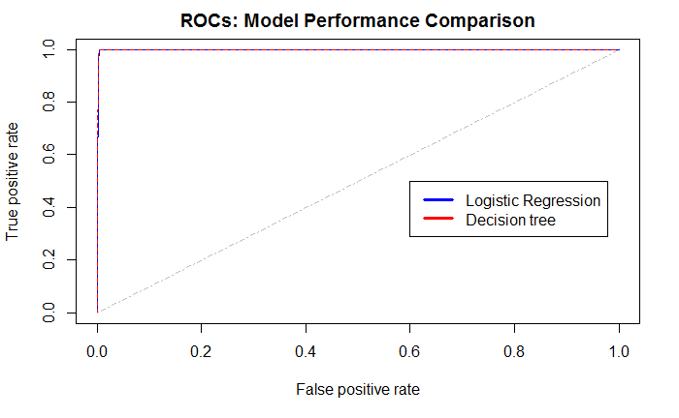
\includegraphics[width=\textwidth]{result0.png}
\centering
\caption{Original Data: ROCs for logistic regression vs decision tree}{\textbf{Source:} Plotted in R Studio}
\label{fig:roc1}
\end{figure}
\end{center}

\begin{center}
\begin{figure}[!htb]
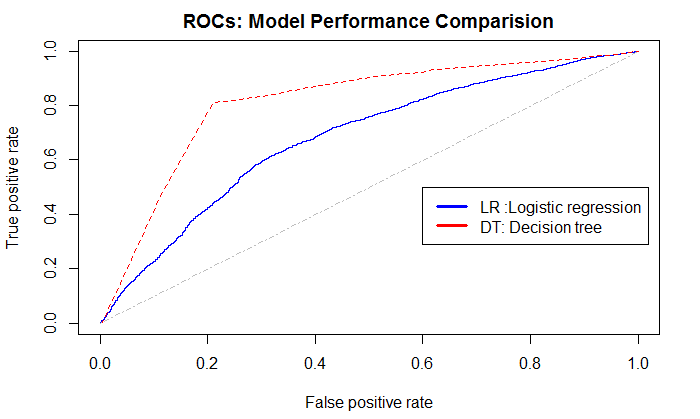
\includegraphics[width=\textwidth]{results1.png}
\centering
\caption{Normalized Data: ROCs for logistic regression vs decision tree}{\textbf{Source:} Plotted in R Studio}
\label{fig:roc}
\end{figure}
\end{center}

Receiver operating characteristic (ROC) is one of technique to estimate the performance of the predictive model by plotting true positive rate(TPR) against the false positive rate(FPR). In figs. \ref{fig:roc} \& \ref{fig:roc1}, performance of logistic regression and decision tree has been compared for ROC index. The original dataset has a 90-degree line for both logistic regression and decision tree, which suggests that predictive might be overfitted. It is evident from the ROC for the normalised data set in fig In \ref{fig:roc} that decision tree performance is better over logistic regression for credit assessment and analysis. In general, higher the area under of ROC (AUROC) curve signifies better performance. \\

Decision tree of original data set is represented in fig.\ref{fig:DTorg}, it can seen that 72\% observations has been classified based on one rule i.e CreditRating <=4.5. Due to this reason original data set was giving accuracy of 99%. 

\begin{center}
\begin{figure}[!htb]
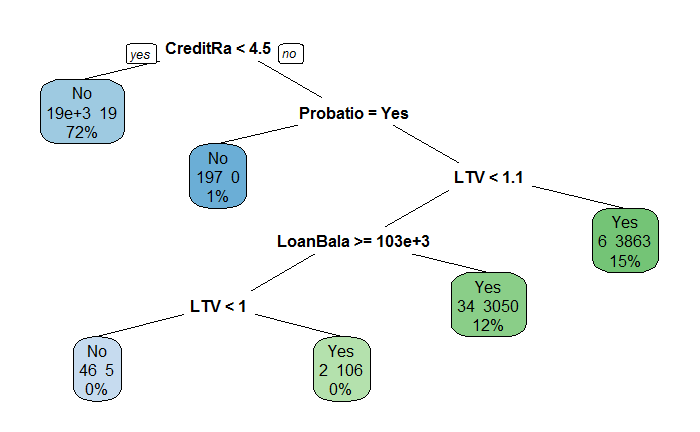
\includegraphics[width=\textwidth]{DTorg.png}
\centering
\caption{Decision tree of original data}{\textbf{Source:} R Package:\citep{rpart.plotpackage}}
\label{fig:DTorg}
\end{figure}
\end{center}

\begin{center}
\begin{figure}[!htb]
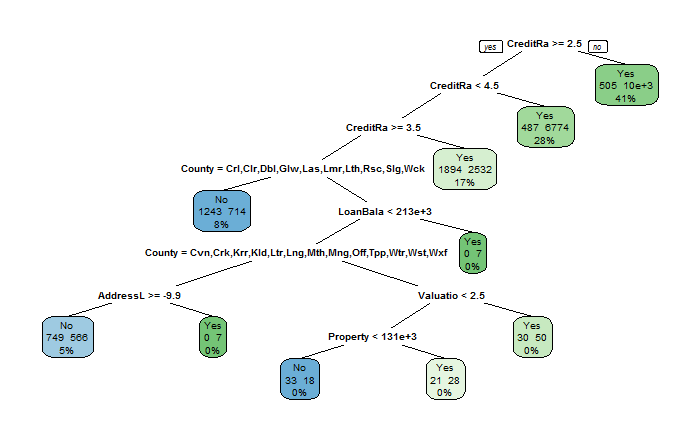
\includegraphics[width=\textwidth]{DTmod.png}
\centering
\caption{Decision tree of modified data}{\textbf{Source:} R Package: \citep{rpart.plotpackage}}
\label{fig:DTmod}
\end{figure}
\end{center}

\begin{center}
\begin{figure}[!htb]
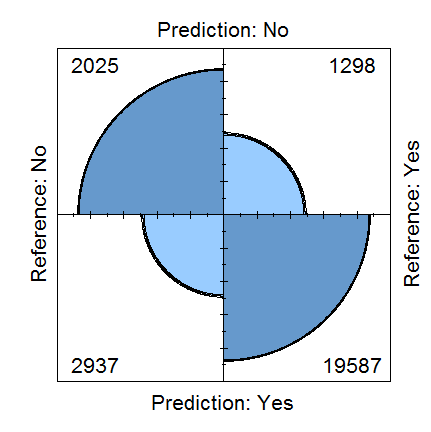
\includegraphics[scale=0.3]{DTcm.png}
\centering
\caption{Confusion Matrix of Test Data}{\textbf{Source:} R Studio}
\label{fig:DTcm}
\end{figure}
\end{center}

In fig. \ref{fig:DTmod}, decision tree for normalized data set is represented and this tree has over 2000 rules which further improves its performance. Due to limitations of page size, we are showing a decision tree with a limited number of nodes. Originally trained tree has 328 nodes and depth of tree was 9. 


\section{Tableau Dashboard}

\begin{center}
\begin{figure}[!htb]
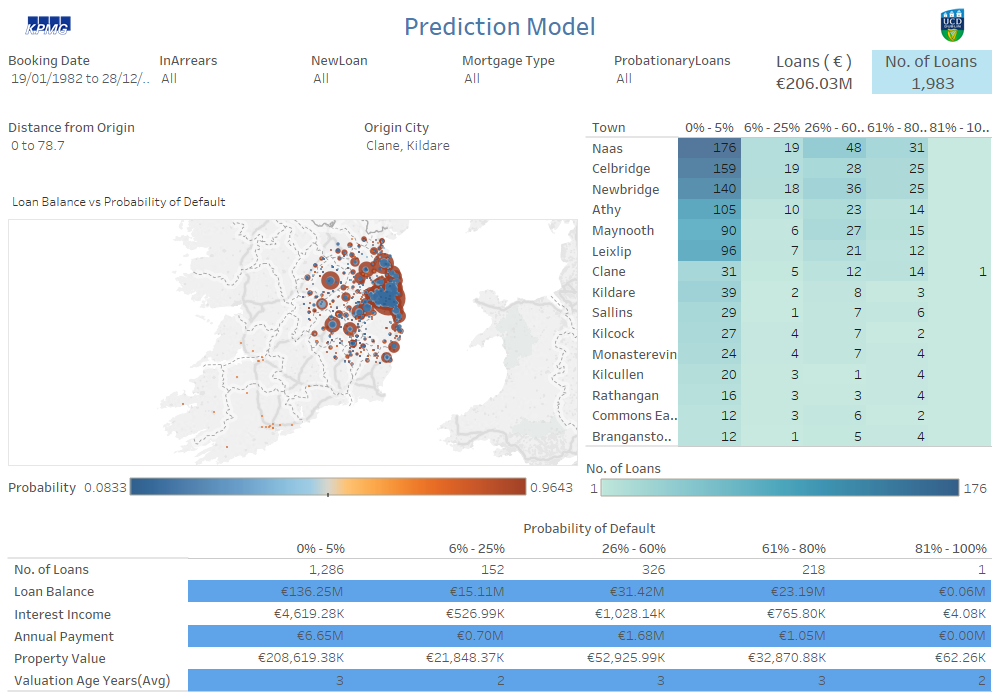
\includegraphics[width=\textwidth]{Predictive.png}
\centering
\caption{Predictive Model Dashboard}{\textbf{Source:} Tableau Professional v10}
\label{fig:overview}
\end{figure}
\end{center}

\subsection{Overview}

Considering the day-to-day requirement of stakeholders at KPMG, three business dashboards are designed using Tableau software. Main response to build dashboard using Tableau,as it allow the easy integrations with predictive model from R engine and provides a better means to visualize prediction and forecast. This dashboard offer an interactive way to identify outlier and analyse loan accounts and user can drill down to street level analyses as shown in fig.\ref{fig.street}. Also, it integrates multiple data sources that turns out to be great time saving for an auditor, as it is not needed to physically map variables from different sources such as employment rate of a town with listed portfolios.\\

\begin{center}
\begin{figure}[!htb]
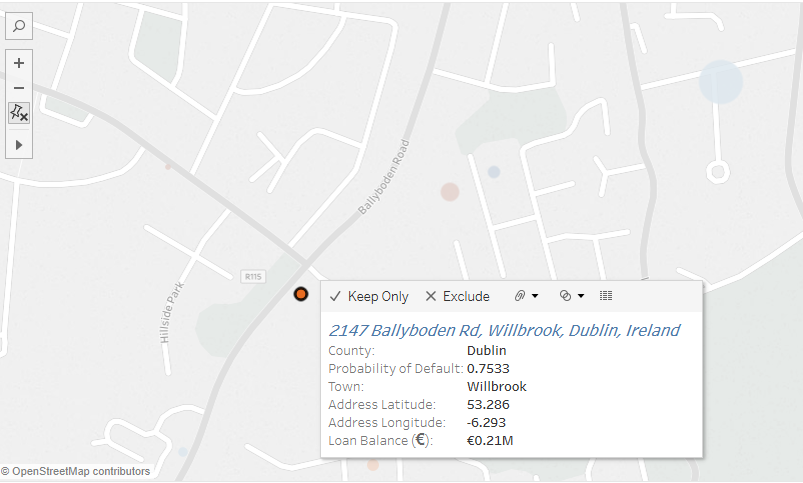
\includegraphics[width=\textwidth]{street.png}
\centering
\caption{Street view map analysis}{\textbf{Source:} Tableau Professional v10}
\label{fig:street}
\end{figure}
\end{center}

\subsection{Predictive Dashboard}

To support end user decision making process, probability of default is segmented into five levels 0-5\%, 6-25\%,26-6\%,61-80\%, and 81-100\%. A heatmap is shown in fig \ref{fig:heatmap}, this will assist credit analyst to find out those loan account which require particular human attention.

\begin{center}
\begin{figure}[!htb]
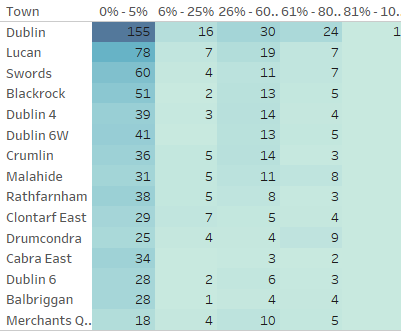
\includegraphics[width=\textwidth]{heatmap.png}
\centering
\caption{Probability Heat map}{\textbf{Source:} Tableau Professional v10}
\label{fig:heatmap}
\end{figure}
\end{center}

\textbf{Case 1:} Division of dashboard into three parts turned out to be good idea as it provides better prediction results: Loan Balance vs Probability of Default, Top fifteen towns and statistical summary table based on selection filter and values. It can be seen from fig. \ref{fig:crash}, number of loans booked during Irish property crash (2007-2010) have highest probability of default.

\begin{center}
\begin{figure}[!htb]
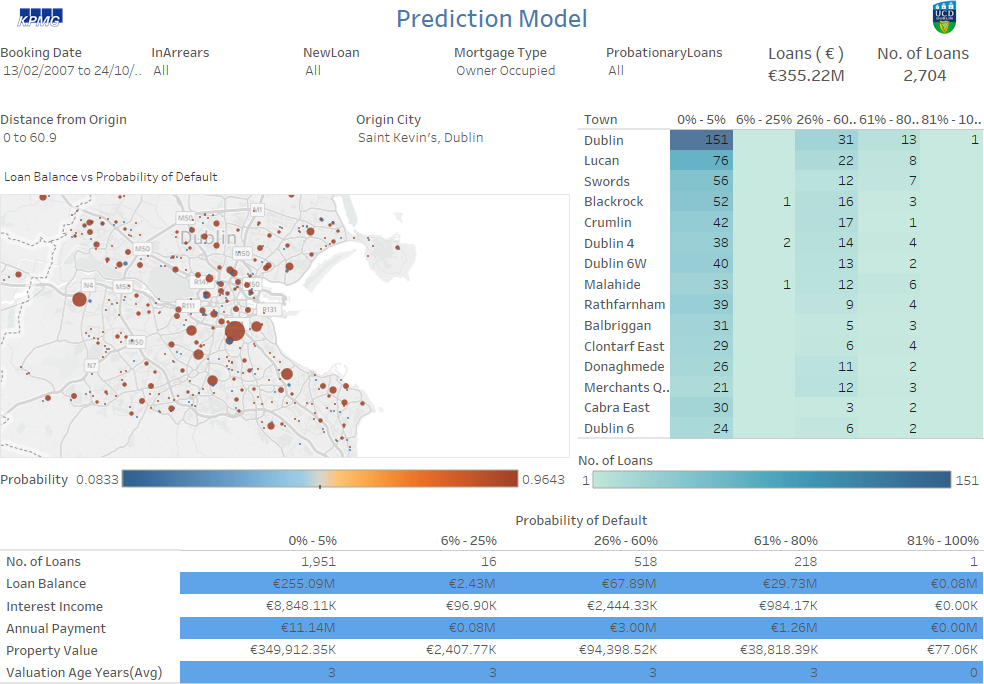
\includegraphics[width=\textwidth]{crash.png}
\centering
\caption{Irish Property Crash analysis}{\textbf{Source:} Tableau Professional v10}
\label{fig:crash}
\end{figure}
\end{center}

\textbf{Case 2:} With use of action filters, dashboard provide detailed information about number of loan account and loan balance due from selected origin city. As in fig. \ref{fig:mala}, there is only one loan account which satisfy selected user criteria. $ 3, Woodlawn, Malahide Demesne, Malahide, Co. Dublin, Ireland$ provability of default is 0.15\% and remaining loan balance is $€0.07M$.  

\begin{center}
\begin{figure}[!htb]
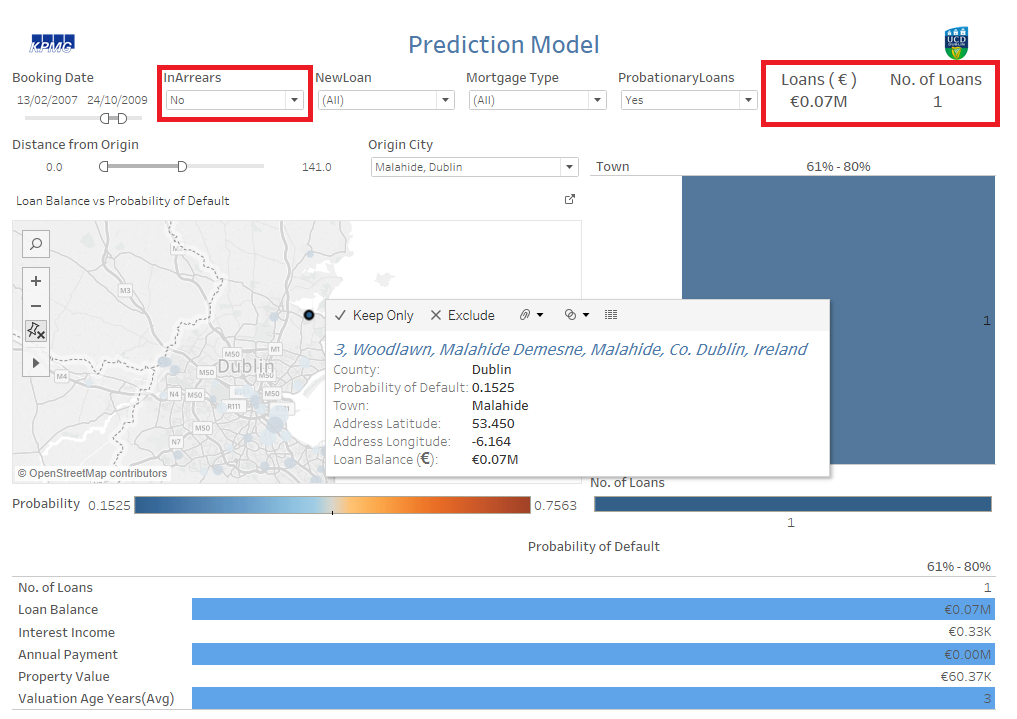
\includegraphics[width=\textwidth]{mala.png}
\centering
\caption{Street view map analysis}{\textbf{Source:} Tableau Professional v10}
\label{fig:mala}
\end{figure}
\end{center}








